\section{Systementwurf}
\label{Systementwurf}
Aus dem Projekt- und Missionsziel leiten sich die folgenden Anforderungen an das System ab.
Um sein Missionsziel zu erfüllen muss sich der Demonstrator bewegen können. Hierfür besitzt er mehrere Antriebsmotoren. Um sein Umfeld wahrzunehmen und das Zielsignal zu erkennen benötigt er Kameras und Abstandssensorik. Außerdem benötigt das System einen Manipulator mit drei Freiheitsgraden um nur durch den Manipulator in allen drei Raumrichtungen mit dem Ziel zu interagieren.
Den Kern des Systems bilden drei STM-32 Mikroprozessoren, die über zwei CAN-Busse miteinander kommunizieren. Zusätzlich zu den Mikroprozessoren hängt noch ein Monitor an den Bussen, der entscheidet welcher Mikroprozessor die Antriebsmotoren über H-Brücken ansteuert.

Im  Blockschaltbild (Abbildung 1) sind alle Grundlegenden Elemente der Hardware und deren Verknüpfung miteinander aufgezeigt.
\begin{figure}[H]
\centering
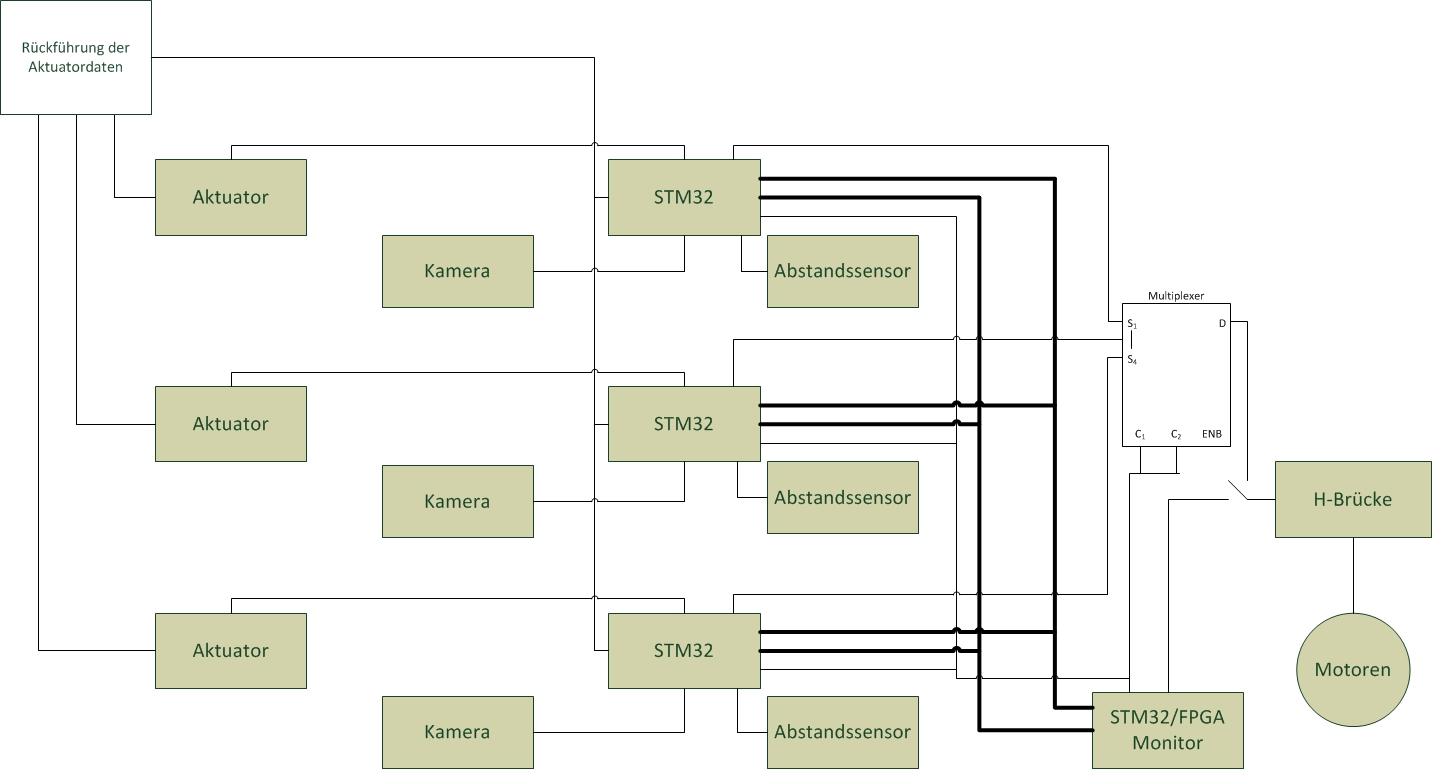
\includegraphics[width=1\linewidth]{Bilder/FaTNet_blockdiagramm.jpg}
\caption{Verknüpfung der Hardware-Elemente} 
\end{figure}
Jeder Mikroprozessor ist für eine Kamera und einen Abstandssensor zuständig und bearbeitet deren Daten. Zusätzlich steuert jeder Mikroprozessor einen Motor des Manipulators und ist somit für einen Freiheitsgrad zuständig. Damit das System unter bestimmten Bedingungen, welche die Freiheitsgrade einschränken, sein Missionsziel noch so gut wie möglich erfüllen kann, hat jeder Mikroprozessor Kenntnis über die Position aller Aktuatoren. Das System ist dadurch in der Lage wegfallende Freiheitsgrade zu kompensieren.

\subsection{Mechanik}
\label{SystementwurfMechanik}
Die Abbildung 2 zeigt die funktionalen Bauteile und deren schematische Anordnung.
Dieser Anordnung zeigt au"serdem die allgemeine Gestalt des Demonstrators, die genauen geometrischen Dimensionen sind noch nicht festgelegt :
\begin{figure}[H]
\centering
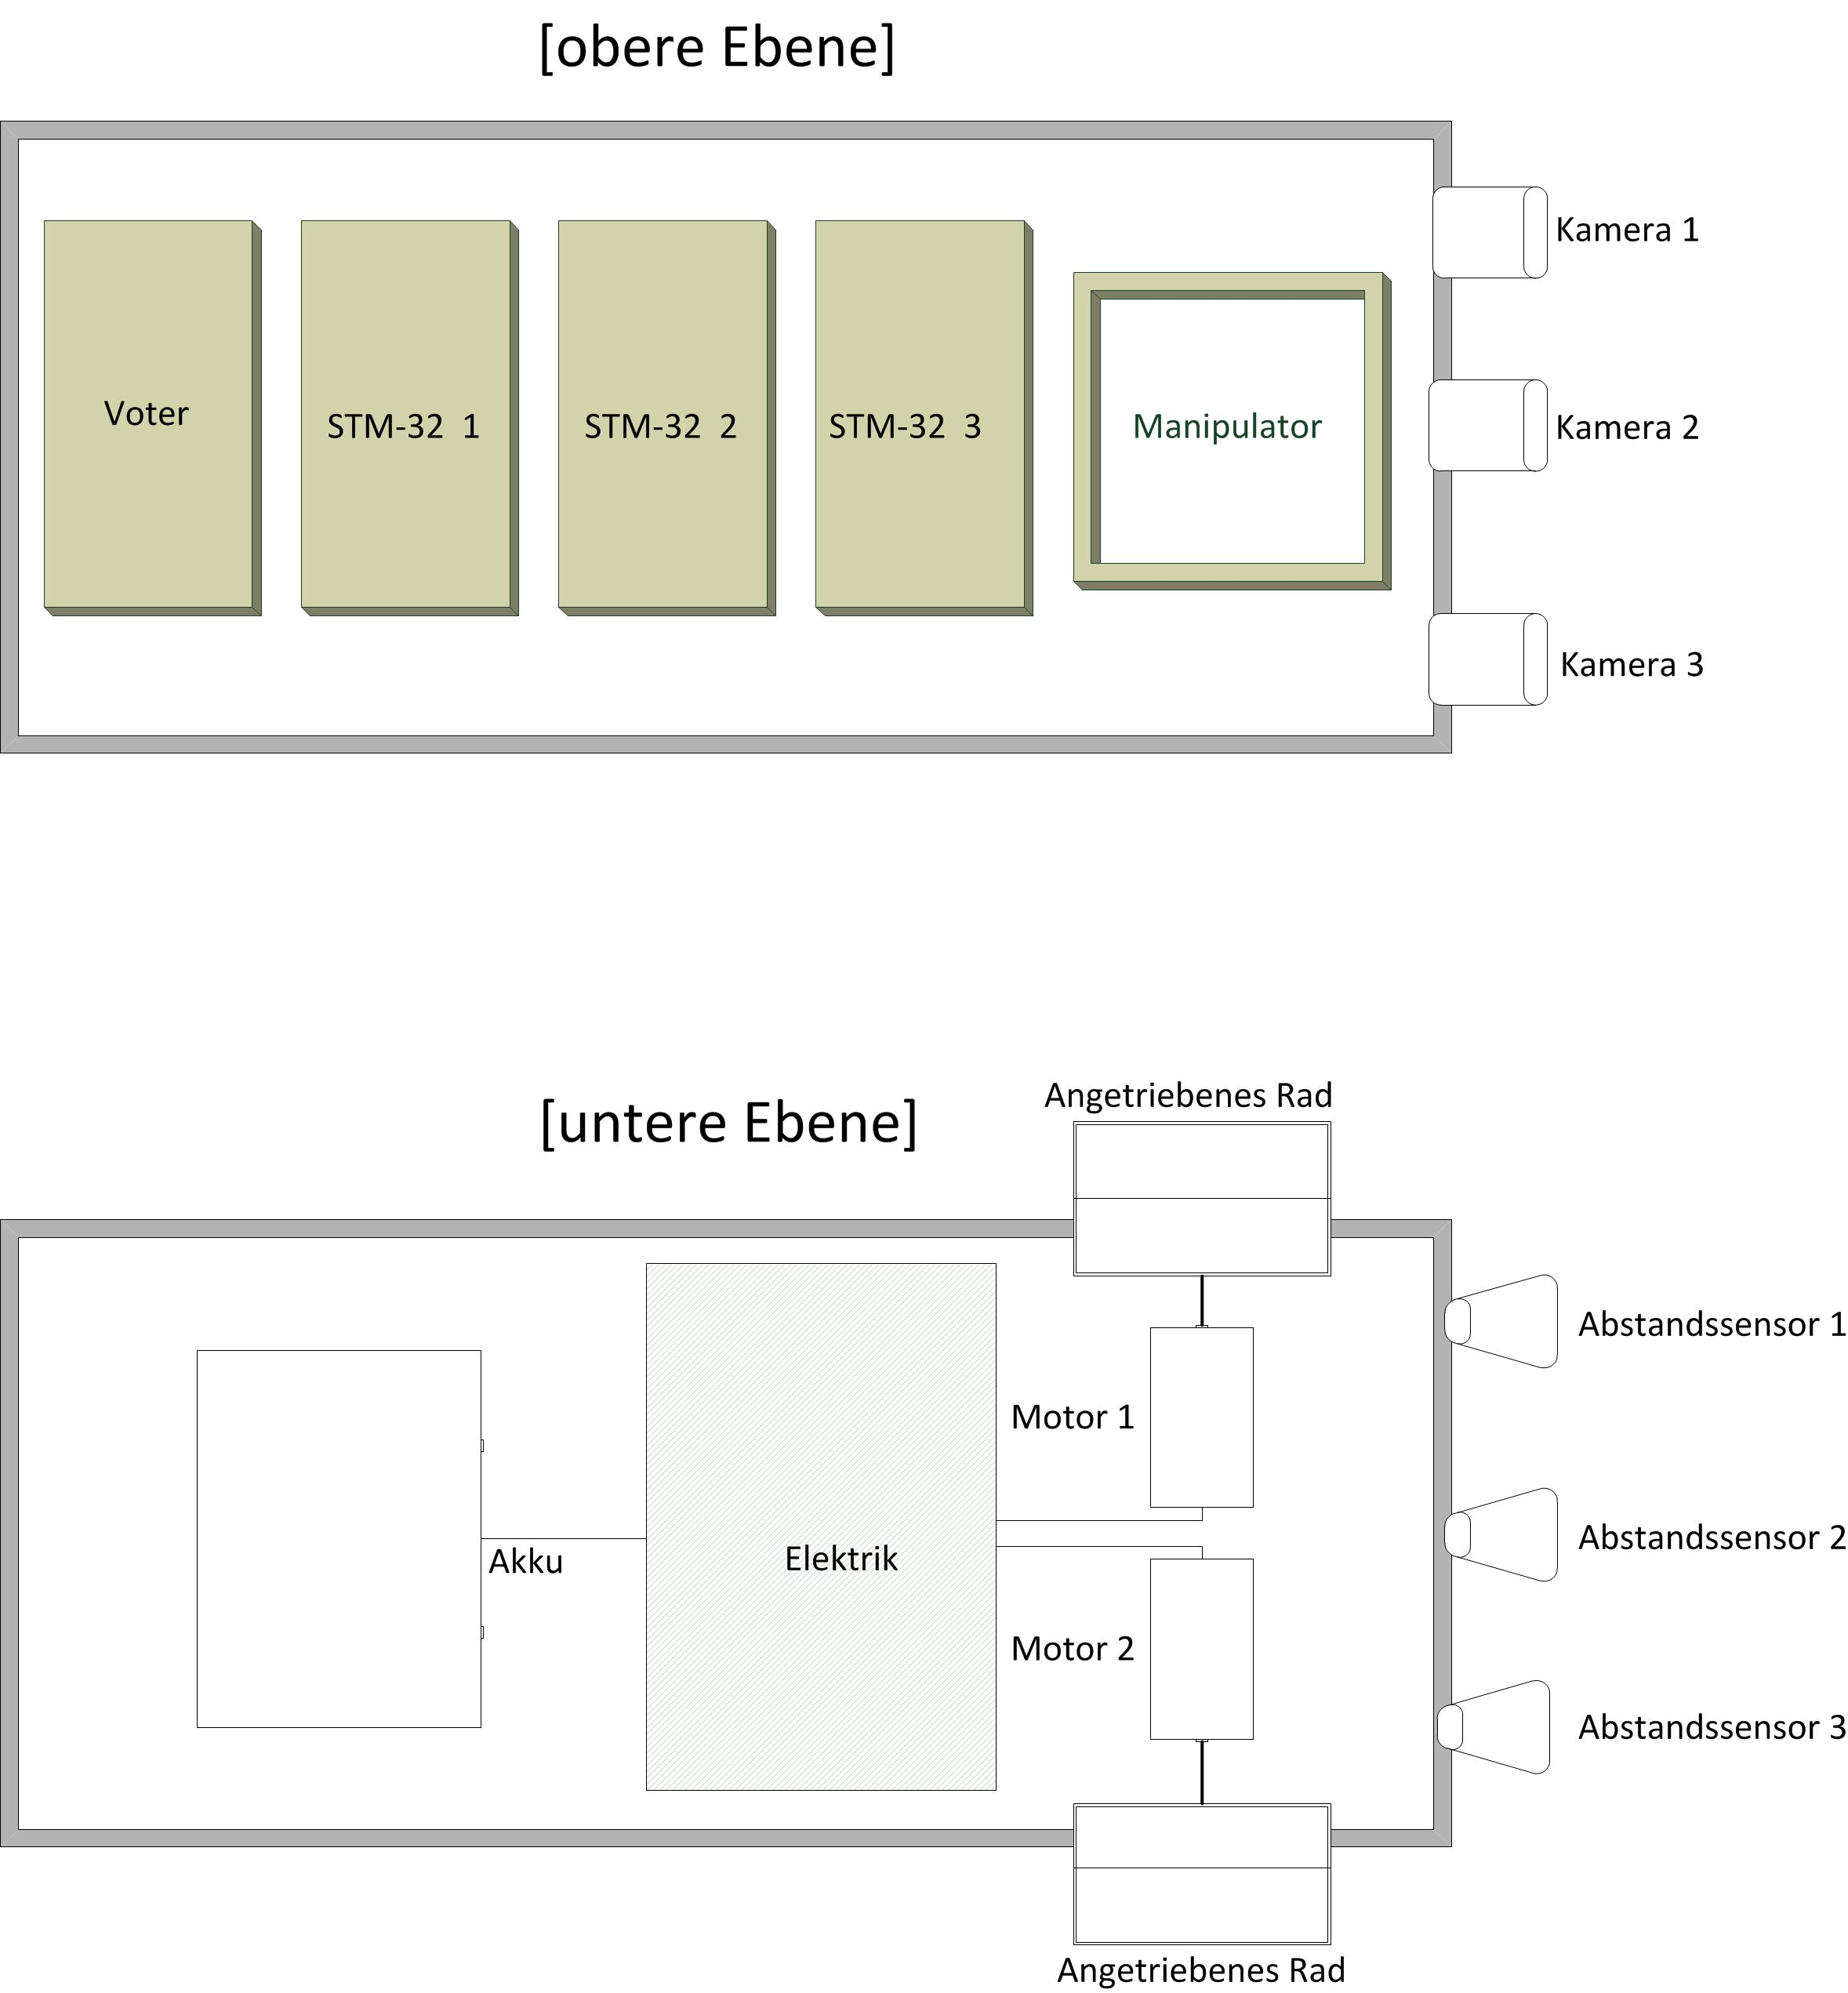
\includegraphics[width=0.7\linewidth]{Bilder/FaTNet_mechanik}
\caption{Anordnung der Komponenten}
\end{figure}
Das Layout der Komponenten ist so vorgesehen, dass alle Elemente auf zwei Ebenen liegen. Würde alternativ jedes STM auf einer separaten Plattform platziert sein oder diese senkrecht aufgestellt werden, wäre es während der Demonstration einerseits schwerer die Fehler am fahrenden System zu injizieren und andererseits wäre nicht genau zu erkennen, welche Fehler injiziert werden.

\subsubsection{Manipulator}
\label{kap:Manipulator}
Am Manipulator sollen die Fehler durch “Graceful degradation” behandelt werden.
Dies bedeutet, dass im Fehlerfall die betroffene Komponente abgeschaltet wird und der Funktionsumfang reduziert wird. Dabei ragt das interagierende Ende in jedem Fall über das Chassis hinaus, so dass, selbst wenn alle Aktuatoren ausfallen, der Arm noch benutzt werden kann.
Fällt nur ein Freiheitsgrad weg, so kann dieser zu einem gewissen Teil durch die Chassis-Konstruktion kompensiert werden:
Die Rotation um die vertikale Achse kann zu einem gewissen Teil durch die Positionierung des Systems ausgeglichen werden.
Fällt ein Aktuator der horizontalen Achse aus wird die Reichweite des Armes eingeschränkt, kann aber durch den zweiten Aktuator in Verbindung mit der Position des Systems ausgeglichen werden.
\begin{figure}[H]
\centering
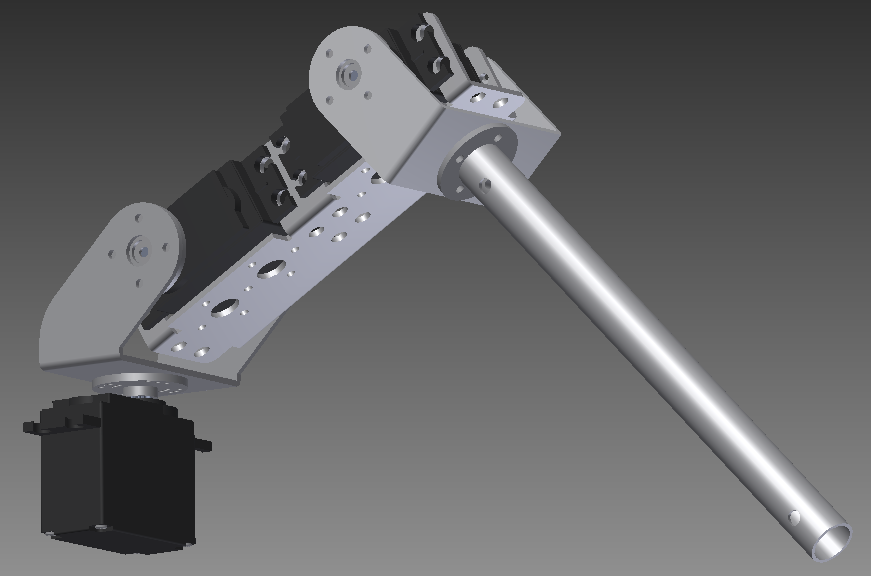
\includegraphics[width=0.5\linewidth]{Bilder/FaTNet_manipulator}
\caption{3D-Entwurf eines Manipulators}
\end{figure}

\subsection{Systementwurf Elektronik}
\label{SystementwurfElektronik}

\subsubsection{Elektrische Leistung}
Die folgende Tabelle zeigt die Komponenten auf, die elektrisch versorgt werden müssen. Die Werte, welche unter Watt eingetragen sind, sind die Worst-Case beötigten Versorgungsleistungen. Unter Umständen wird ein LC-Display benötigt, dahe rwird es mit aufgeführt. Unter Anzahl ist angegeben wieviele dieser Komponenten maximal im System verbaut werden.
Sind konkrete Komponenten angegeben so handelt es sich um Vorschläge die im Rahmen dieser Überschlagsrechnung Sinn ergeben.
\begin{table}[H]
\centering
\begin{tabular}{|c|c|c|}
\hline 
\textbf{Verbraucher} & \textbf{Maximale Leistungsaufnahme in Watt} & \textbf{Anzahl} \\ 
\hline 
Motor & 17 & 2 \\ 
\hline 
Mikrocontroller & 2.5 & 4 \\ 
\hline 
Kamera (OV7670) & 0.06 & 3 \\ 
\hline 
Display & 0.056 & 3 \\ 
\hline 
Servomotor & 2.7 & 4 \\ 
\hline 
\end{tabular}
\caption{Abschätzung des Leistungsbedarfs der Elektronik-Komponenten}
\label{tab:leistung}
\end{table} 
In der Summe ergibt sich ein Leistungsbedarf von rund 53 Watt. Eine Laufzeit von einer Stunde wird als erstrebenswert angesehen. Daraus resultiert eine benötigte Energiemenge von 53 Wattstunden.

\subsubsection{Energiespeicher}
Es werden LiFePo4-Akkumulatoren als Energiequelle verwendet werden.
%Ein Akku aus drei Zellen (11,1 Volt Nennspannung) müsste eine Kapazität von 4,8 Amperestunden besitzen, um die oben %aufgestellte Laufzeitanforderung zu erfüllen. Bei einem vierzelligen Akku (14,8 V) wären es 3,6 Amperestunden.

\subsection{Software}
Im folgenden Abschnitt wird grob auf die Softwarearchitektur eingegangen. Es wird erklärt, wie sich das System nach dem Einschalten verhält, an welcher Stelle die essentiellen Aktionen ausgeführt werden und an welchen Stellen dabei Fehler auftreten können. Von der Beschreibung der jeweils unterliegenden Algorithmen wird an dieser Stelle abgesehen.
Die Programmierung der verwendeten STM32-Mikrocontroller erfolgt in C++. Dabei wird auf die XPCC-Library (Cross Platform Component Communication) zurückgegriffen.

\subsubsection{Grundstruktur}
Nachdem der Mikrocontroller mit Spannung versorgt wird und gebootet ist, wird mit der Initialisierung der einzelnen Softwaremodule begonnen. Geplant sind folgende Module: 
\paragraph{CAN-Bus und  Protokoll}$\;$\\
Dieses Modul dient zur Kommunikation zwischen den verschiedenen STM-Boards. Dabei bildet der CAN-Bus das grundlegende Kommunikationsinterface. Auf dieses wird ein an der Problemstellung angepasstes Protokoll aufgesetzt. Eine funktionierende Kommunikation ist Voraussetzung um am Netzwerk teilzunehmen.

\paragraph{Heartbeat}$\;$\\
Durch den Heartbeat wird den übrigen Komponenten mitgeteilt, dass der Absender im Netzwerk zur Verfügung steht. Gegebenfalls können Fehler, die bei einem Teilnehmer auftreten, übermittelt werden. Ist es nicht möglich einen Heartbeat zu senden wird davon ausgegangen das keine Kommunikation vorhanden ist und es kommt zu einer  Fehlerbehandlung. Solange ein Heartbeat über das Netzwerk empfangen kann mit den Absender kommuniziert werden.

\paragraph{SysTick}$\;$\\
Der SysTick-Handler wird in fest definierten Zeitabständen per Interrupt aufgerufen. Im Handler werden Aufgaben ausgeführt die in regelmäßigen Abständen von Nöten sind. Beispielsweise die Regelung und der Heartbeat.

\paragraph{Kamera/Bildverarbeitung}$\;$\\
Die Kamera und die Verarbeitung der resultierenden Bilder wird zur Orientierung in der Umwelt verwendet. Nachdem die Informationen mittels Segmentierung, Klassifizierung und Positionbestimmung aus dem Bild extrahiert wurden, werden diese mit denen der anderen Teilnehmern verglichen um die Plausibilität zu prüfen. Die Informationen werden anschließend an den Wegplaner übergeben. Ist die Markierung in Reichweite wird von einer weiteren Wegplanung abgesehen. Stattdessen wird die Steuerung für den Roboterarm aufgerufen.

\paragraph{Abstandssensoren}$\;$\\
Dienen zur Vermeidung von Kollisionen. Deren Werte fließen ebenfalls in der Wegplanung mit ein.

\paragraph{Antrieb/ Regelung}$\;$\\
Die Regelung wird regelmäßig im SysTick-Handler ausgeführt. Die durch die Trajektorie vorgegebenen Soll-Werte werden mit den Ist-Werten der Encoder, welche die Drehzahl der Motoren zurückgeben, verglichen und gegebenfalls korrigiert. Der Voter legt in gleichmäßigen Zeitabständen einen Mikrocontroller als Master fest, der die Motoren regelt.

\paragraph{Roboterarm}$\;$\\
Befindet sich das System in der Position, dass der Manipulatior mit dem Ziel interagieren kann wird von der Wegplanung auf die Manipulatorsteuerung umgeschaltet. Die Winkelvorgabe der Aktuatoren geschieht per inverser Kinematik. Dabei müssen für den Ausfall von Aktuatoren mehrere Kinematik vorhanden sein, um das Ziel weiterhin zu erreichen.
 
\begin{figure}[H]
\centering
  \begin{minipage}[b]{0.49\linewidth}
    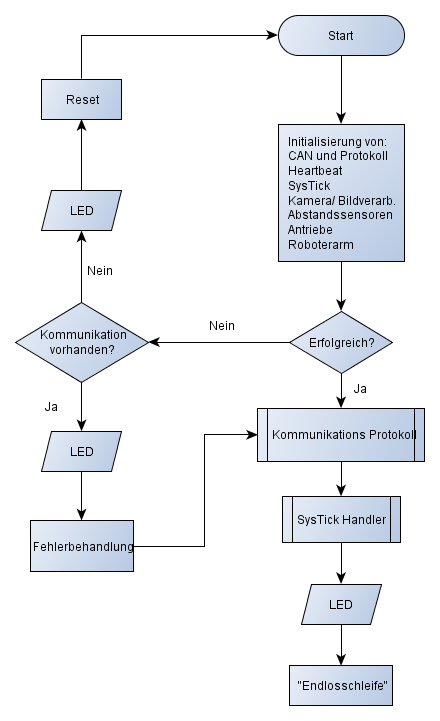
\includegraphics[width=\linewidth]{Bilder/FaTNet_init} 
    \caption{Flussdiagramm zur Initialisierung }
    \label{fig:init}
  \end{minipage}
  \begin{minipage}[b]{0.49\linewidth}
    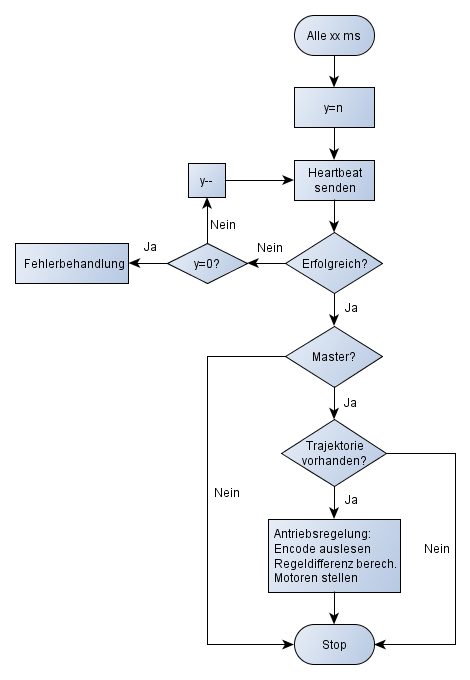
\includegraphics[width=\linewidth]{Bilder/FaTNet_systick}  
    \caption{Flussdiagramm zum SysTick-Handler}
    \label{fig:systick}
  \end{minipage}
\end{figure}

\begin{figure}[H]
\centering
    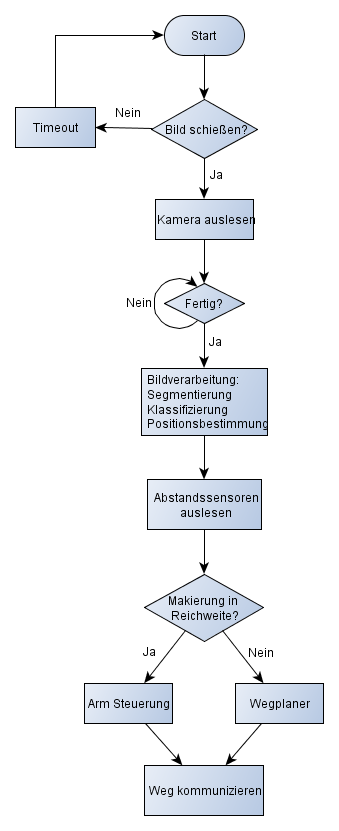
\includegraphics[width=0.4\linewidth]{Bilder/FaTNet_schleife}  
    \caption{Flussdiagramm zum Softwareablauf}
    \label{fig:schleife}
\end{figure}
